\label{Chapter:Automated Guided Jumping}
In this chapter we will start by discussing the interaction design for an automated guided jumping navigation technique that would meet the research questions referenced in \ref{section:GJM Conclusion}. This will be followed by details about development of the technique which can be divided into three parts; the setup of an environment and narrative structure for using this technique, development of automated jumping and finally how to make the jumps comprehensible to users. 

\section{Interaction Design}
\label{section AGJ: Interaction Design}
Looking at the use cases and motivation discussed in Chapter \ref{Chapter:Guided Jumping Motivation} we will first lay out a scenario in which our technique would be used and then go through the interaction design of the technique based on this scenario.

\subsection{Scenario}
\label{subsection AGJ ID: Scenario}
We developed our automated guided jumping navigation technique  for a virtual tour of an indoor space which a user can do alone without a tour guide. There is potential to think of how this can be extended to a virtual tour of an indoor space for a group of users without a tour guide as well. The goal of this virtual tour would be to explore specific objects and exhibits that could have a similar theme that a user is interested it and learn about them while also remembering what they have seen and where they saw it. 

\subsection{Exploration Steps}
\label{subsection AGJ ID: Exploration Steps}
A tour of the \acrshort{ve} would take place by ensuring that users go to specified locations of interest or nodes. Since these could be quite far from each other there should be way points in between each node so that users would travel shorter distances to the nodes, hence, justifying the navigation being a jumping metaphor instead of teleportation. As shown in Figure \ref{fig:interaction-design-steps}, when a user is touring the environment they start at the first node. Here they can explore and wait for a while till they are willing to move on. When they are ready to jump they get some form of travel feedback so they are aware that a jump is about to take place. Then a jump takes place to either the next node or a way point. The user can no explore and wait or again jump to the next node or way point. The jumps would keep taking place until the final node is reached and the tour ends. 

\begin{figure}[]
	\centering
	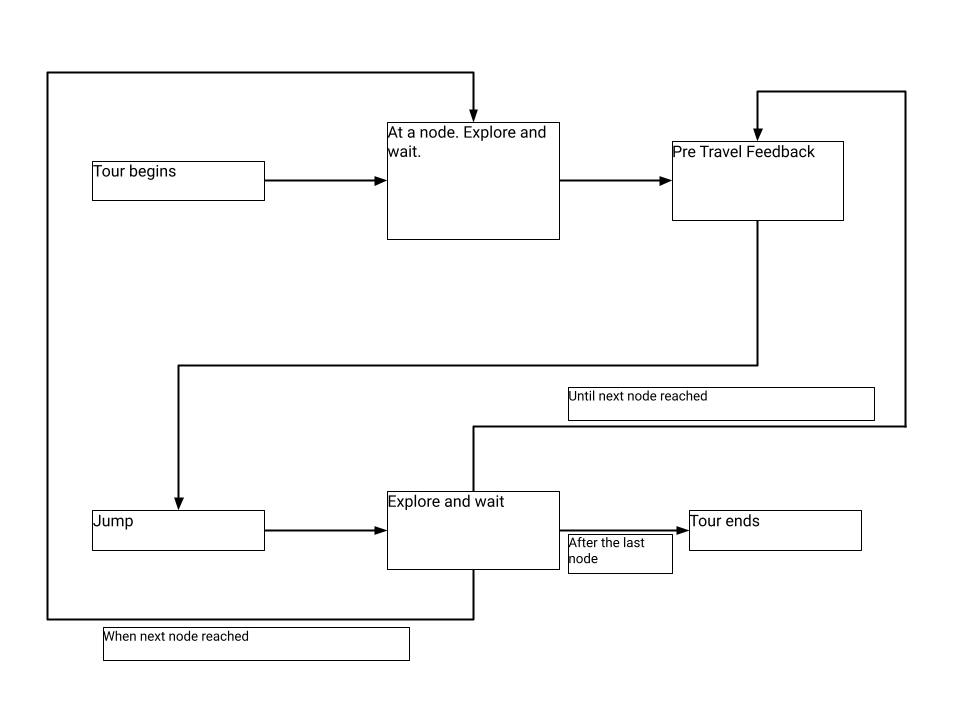
\includegraphics[width=0.5\textwidth]{images/interaction-design-steps.png}
	\caption{Steps that would be followed in an exploration of a \acrshort{ve} using the automated guided jumping navigation technique.}
	\label{fig:interaction-design-steps}
\end{figure}

\subsubsection{Travel Feedback}
\label{subsubsection AGJ ID ES: Travel Feedback}
Before a jump takes place, a user needs to know the following information:
\begin{itemize}
	\item The location they will jump to.
	\item Their orientation after the jump.
	\item The time left until the jump takes place.
	\item Whether or not a jump is paused, giving them time to explore.
\end{itemize}

\subsubsection{Pause to Explore}
\label{subsubsection AGJ ID ES: Pause to Explore}
As the jumping is done automatically, it is important to provide the user with some way to control the technique. This can be done by allowing them to somehow pause the jumping either implicitly or explicitly so that they can take the time to explore or look around rather than being worried about automatically moving to the next position. Similarly, users would then also have the ability to implicitly or explicitly to resume once they are ready to continue.

\subsubsection{Choice between Nodes}
\label{subsubsection AGJ ID ES: Choice between Nodes}
In addition to users having the option to pause, users should also have some control over the path they take. This can be provided by adding some nodes where a choice is given to the users between multiple possible nodes they can go to. Information and travel feedback about each node is given to the users and then they can select their preferred node from the given options. 

\section{Environment Setup}
\label{section AGJ: Environment Setup}

Once we came up with a suitable interaction design for the technique
\begin{figure}[]
	\centering
	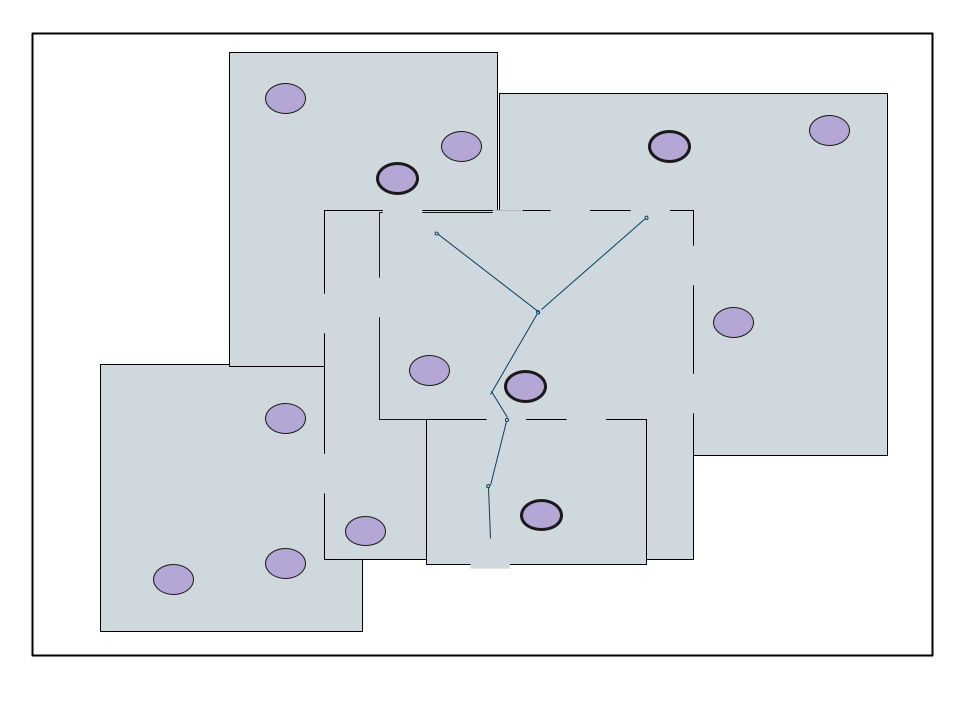
\includegraphics[width=0.5\textwidth]{images/interaction-design-layout.png} %replace with picture of actual environment on unity with visible nodes
	\caption{This is a potential setup of an environment in which the automated guided jumping navigation would be used. Black spheres = nodes, yellow spheres = way points, arrows and numbers where there is a choice between nodes}
	\label{fig:interaction-design-layout}
\end{figure}
\section{Automated Jumping}
\label{section AGJ: Automated Jumping}
%\section{Gesture Control}
%\label{section AGJ: Gesture Control}
\section{Comprehensibility of Jumps}
\label{section AGJ: Comprehensibility of Jumps}